\chapter{Instrukcja użytkowania}
\section{Krótki opis pirometru i jego przeznaczenia}

Poniższy pirometr jest projektem naukowo-badawczym, służącym do bezkontaktowego pomiaru temperatury oraz wyświetlania jej w czasie rzeczywistym na wbudowanym wyświetlaczu LCD. Urządzenie oferuje możliwość wyboru wyświetlania temperatury według skali Celsjusza, Fahrenheita oraz Kelwina. Ponadto, miernik umożliwia dostosowanie emisyjności w zakresie od 0.00 do 1.00.

\vspace{12pt}

Obudowa urządzenia jest niepełna, charakteryzująca się prostym, schludnym i nowoczesnym wyglądem. Ze względu na delikatne elementy, urządzenie jest nieodpowiednie do użytkowania przez dzieci. Posiada klasę odporności IP10, co oznacza, że nie należy narażać go na kontakt ze skutkami opadów atmosferycznych oraz przypadkowym zalaniem. Czyszczenie urządzenia powinno odbywać się z użyciem ściereczki nasączonej wodą, ewentualnie z dodatkiem delikatnego detergentu. W przypadku uszkodzenia urządzenia lub jego nieprawidłowego działania, należy skontaktować się z producentem lub oddać urządzenie do punktu naprawczego.

\newpage

Urządzenie składa się z następujących elementów:
\begin{itemize}
    \item dwóch paneli poliwęglanowych o grubości 3 mm stanowiących obudowę,
    \item płyty ewaluacyjnej,
    \item modułu Arduino Uno pełniącego rolę serca urządzenia,
    \item czujnika pirometrycznego,
    \item klawiatury,
    \item wyświetlacza LCD.
\end{itemize}

\section{Dane techniczne}
\begin{itemize}
    \item \textbf{Prędkość próbkowania:} 1/sekundę,
    \item \textbf{Zasilanie:} USB-B 5V,
    \item \textbf{Pobór prądu:} >50 mA,
    \item \textbf{Klasa odporności:} IP10,
    \item \textbf{Zakres pomiaru temperatury:} od -30 do 150~$^{\circ}$C,
    \item \textbf{Dopuszczalna wilgotność względna bez kondensacji:} 5--95\%,
    \item \textbf{Temperatura pracy oraz przechowywania:} od -10 do 50~$^{\circ}$C,
    \item \textbf{Wymiary:} 160~x~200 mm,
    \item \textbf{Waga:} 350 g.
\end{itemize}

\newpage

\section{Obsługa urządzenia}
Po podłączeniu urządzenia do zasilania za pomocą kabla USB-B, jest ono natychmiast gotowe do pracy i wykonuje pomiary. Należy skierować przednią część urządzenia (w której znajduje się element pomiarowy) na badany obiekt. Wyniki pomiarów są wyświetlane na ekranie LCD w czasie rzeczywistym.

\vspace{12pt}

Ustawienie emisyjności w zakresie od 0.00 do 1.00 odbywa się za pomocą klawiszy \texttt{EMISYJN. +} oraz \texttt{EMISYJN. -}. Tabela emisyjności typowych materiałów znajduje się na rysunku 4. Prawidłowe ustawienie emisyjności ma istotny wpływ na dokładność pomiarów i powinno być dostosowywane przy każdej zmianie badanej powierzchni. W celu przywrócenia wartości domyślnej emisyjności (1.00), należy użyć przycisku \texttt{EMISYJN. RESET}.

\vspace{12pt}

Zmianę skali temperatury pomiędzy stopniami Celsjusza, Fahrenheita oraz Kelwina wykonuje się przyciskiem \texttt{°C / °F}. Po zakończeniu pomiarów należy odłączyć przewód zasilający od urządzenia. Pirometr powinien być przechowywany w suchym miejscu.

\section{Opis budowy urządzenia}

Rys.1 przedstawia panel górny urządzenia. Najważniejsze jego elementy to:

\begin{enumerate}
    
    \item Element pirometryczny służący do pomiaru temperatury.
    
    \item Moduł Arduino Uno z gniazdem zasilającym urządzenie oraz interfejsem USB-C.
    
    \item Wyświetlacz LCD z niebieskim podświetleniem.
    
    \item Klawiatura służąca do wprowadzania ustawień urządzenia.

\end{enumerate}

\begin{figure}[h!]
    \centering
    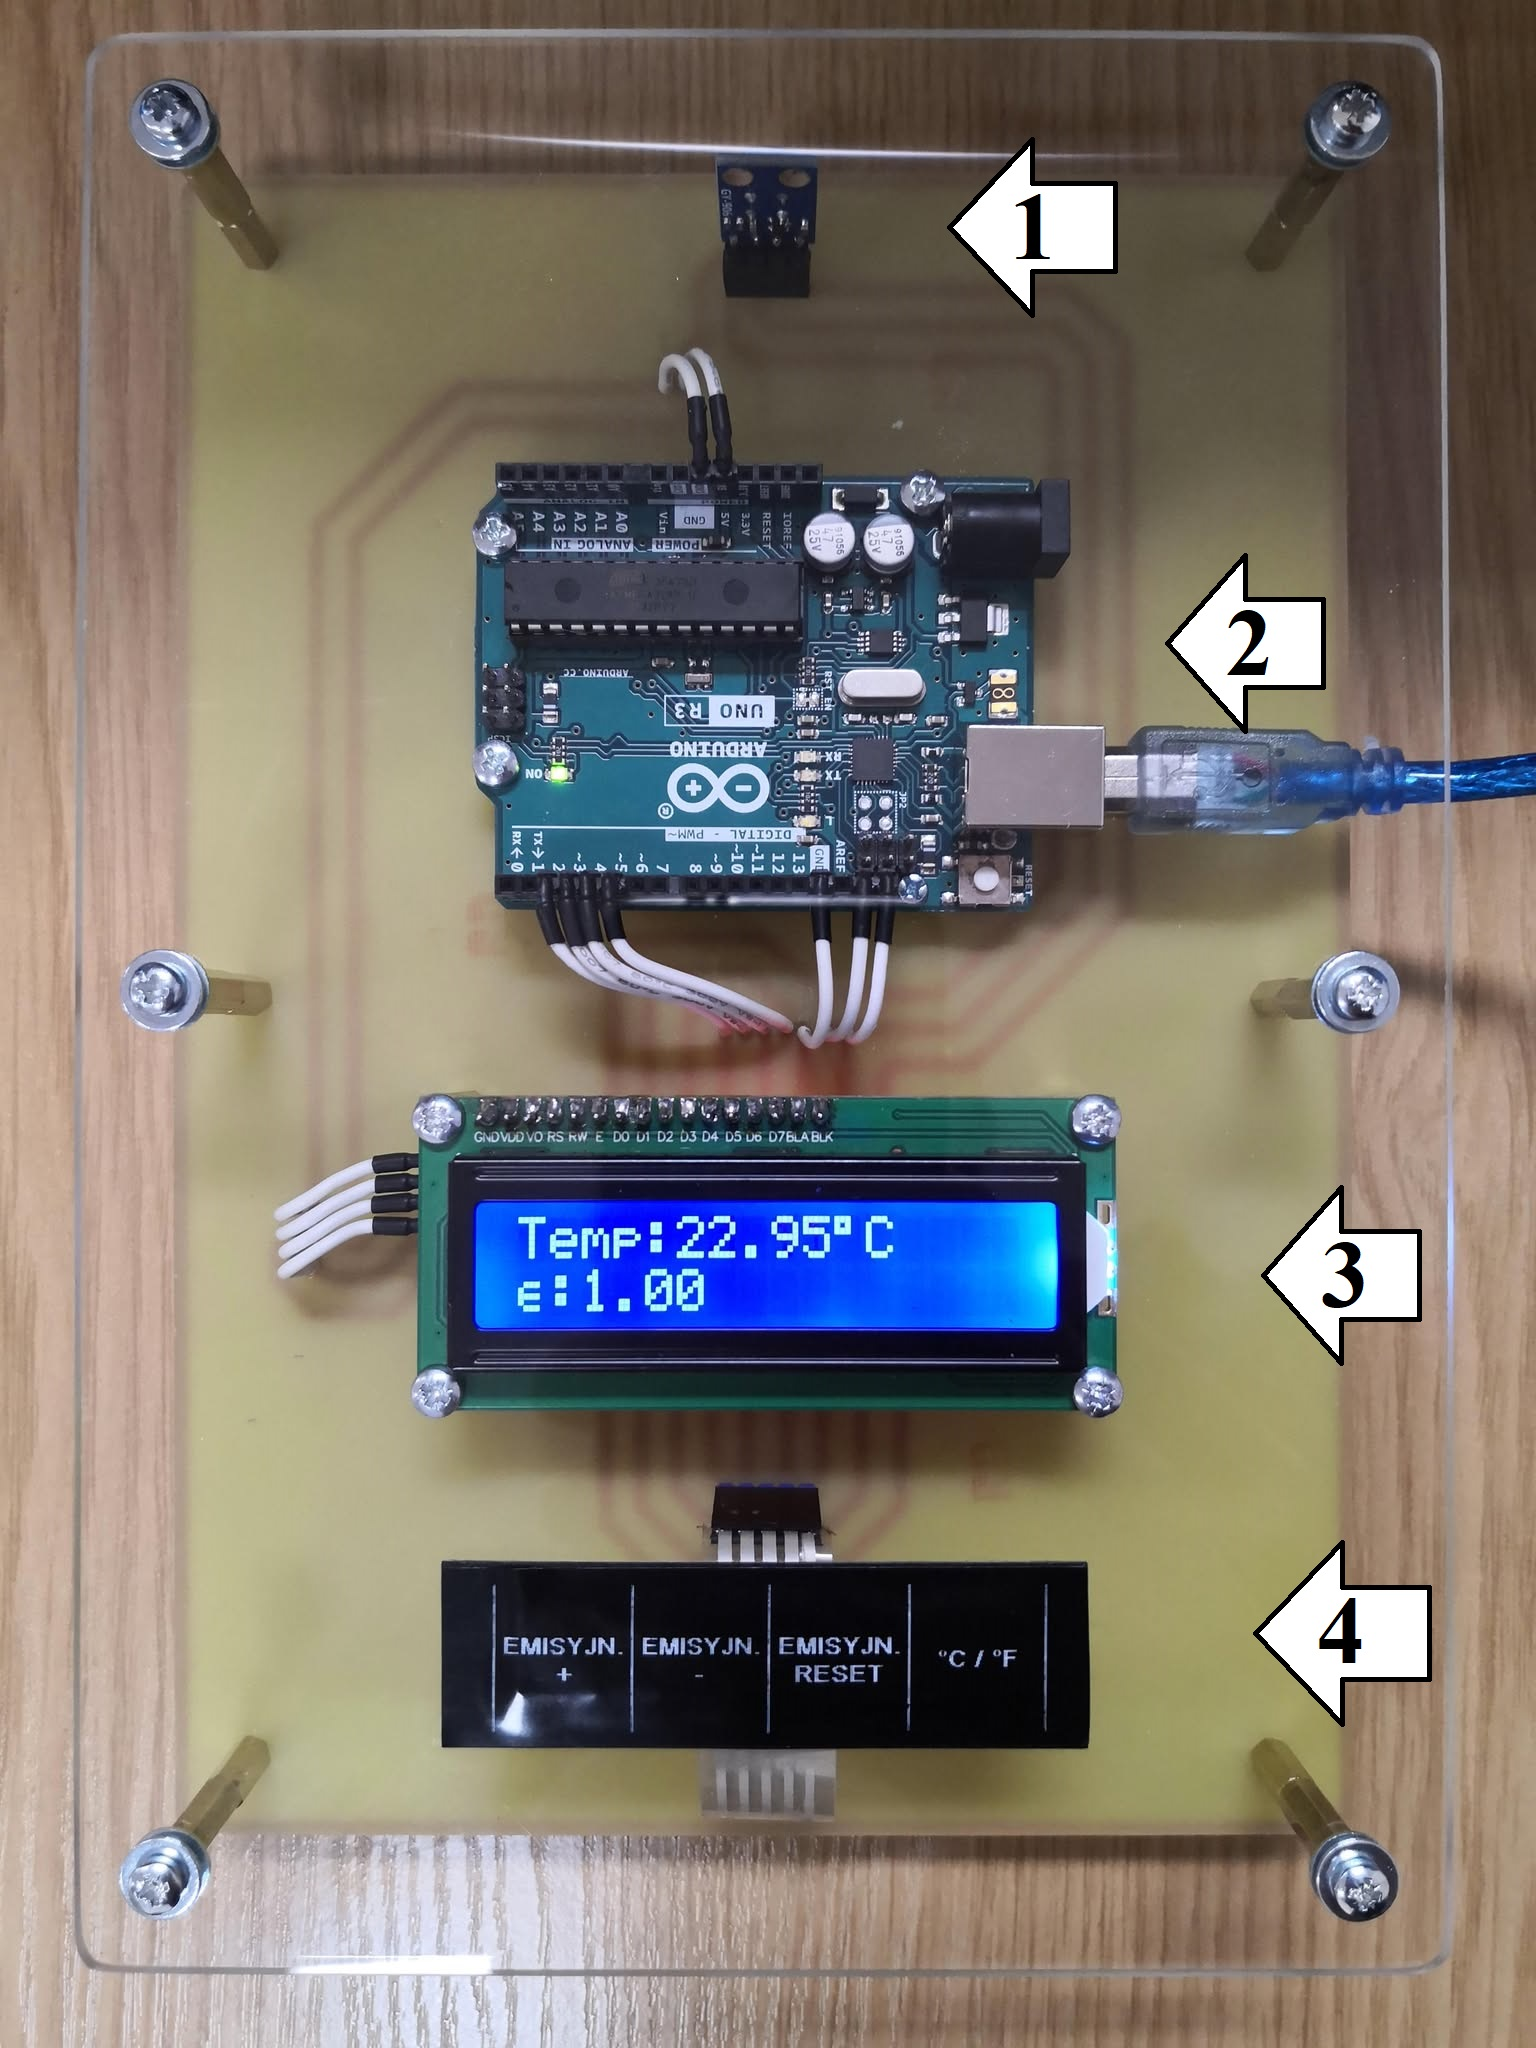
\includegraphics[width=0.9\textwidth]{images/front_opis.jpg}
    \caption{Panel górny urządzenia}
    \label{fig:panel_gorny}
\end{figure}

\begin{figure}[h!]
    \centering
    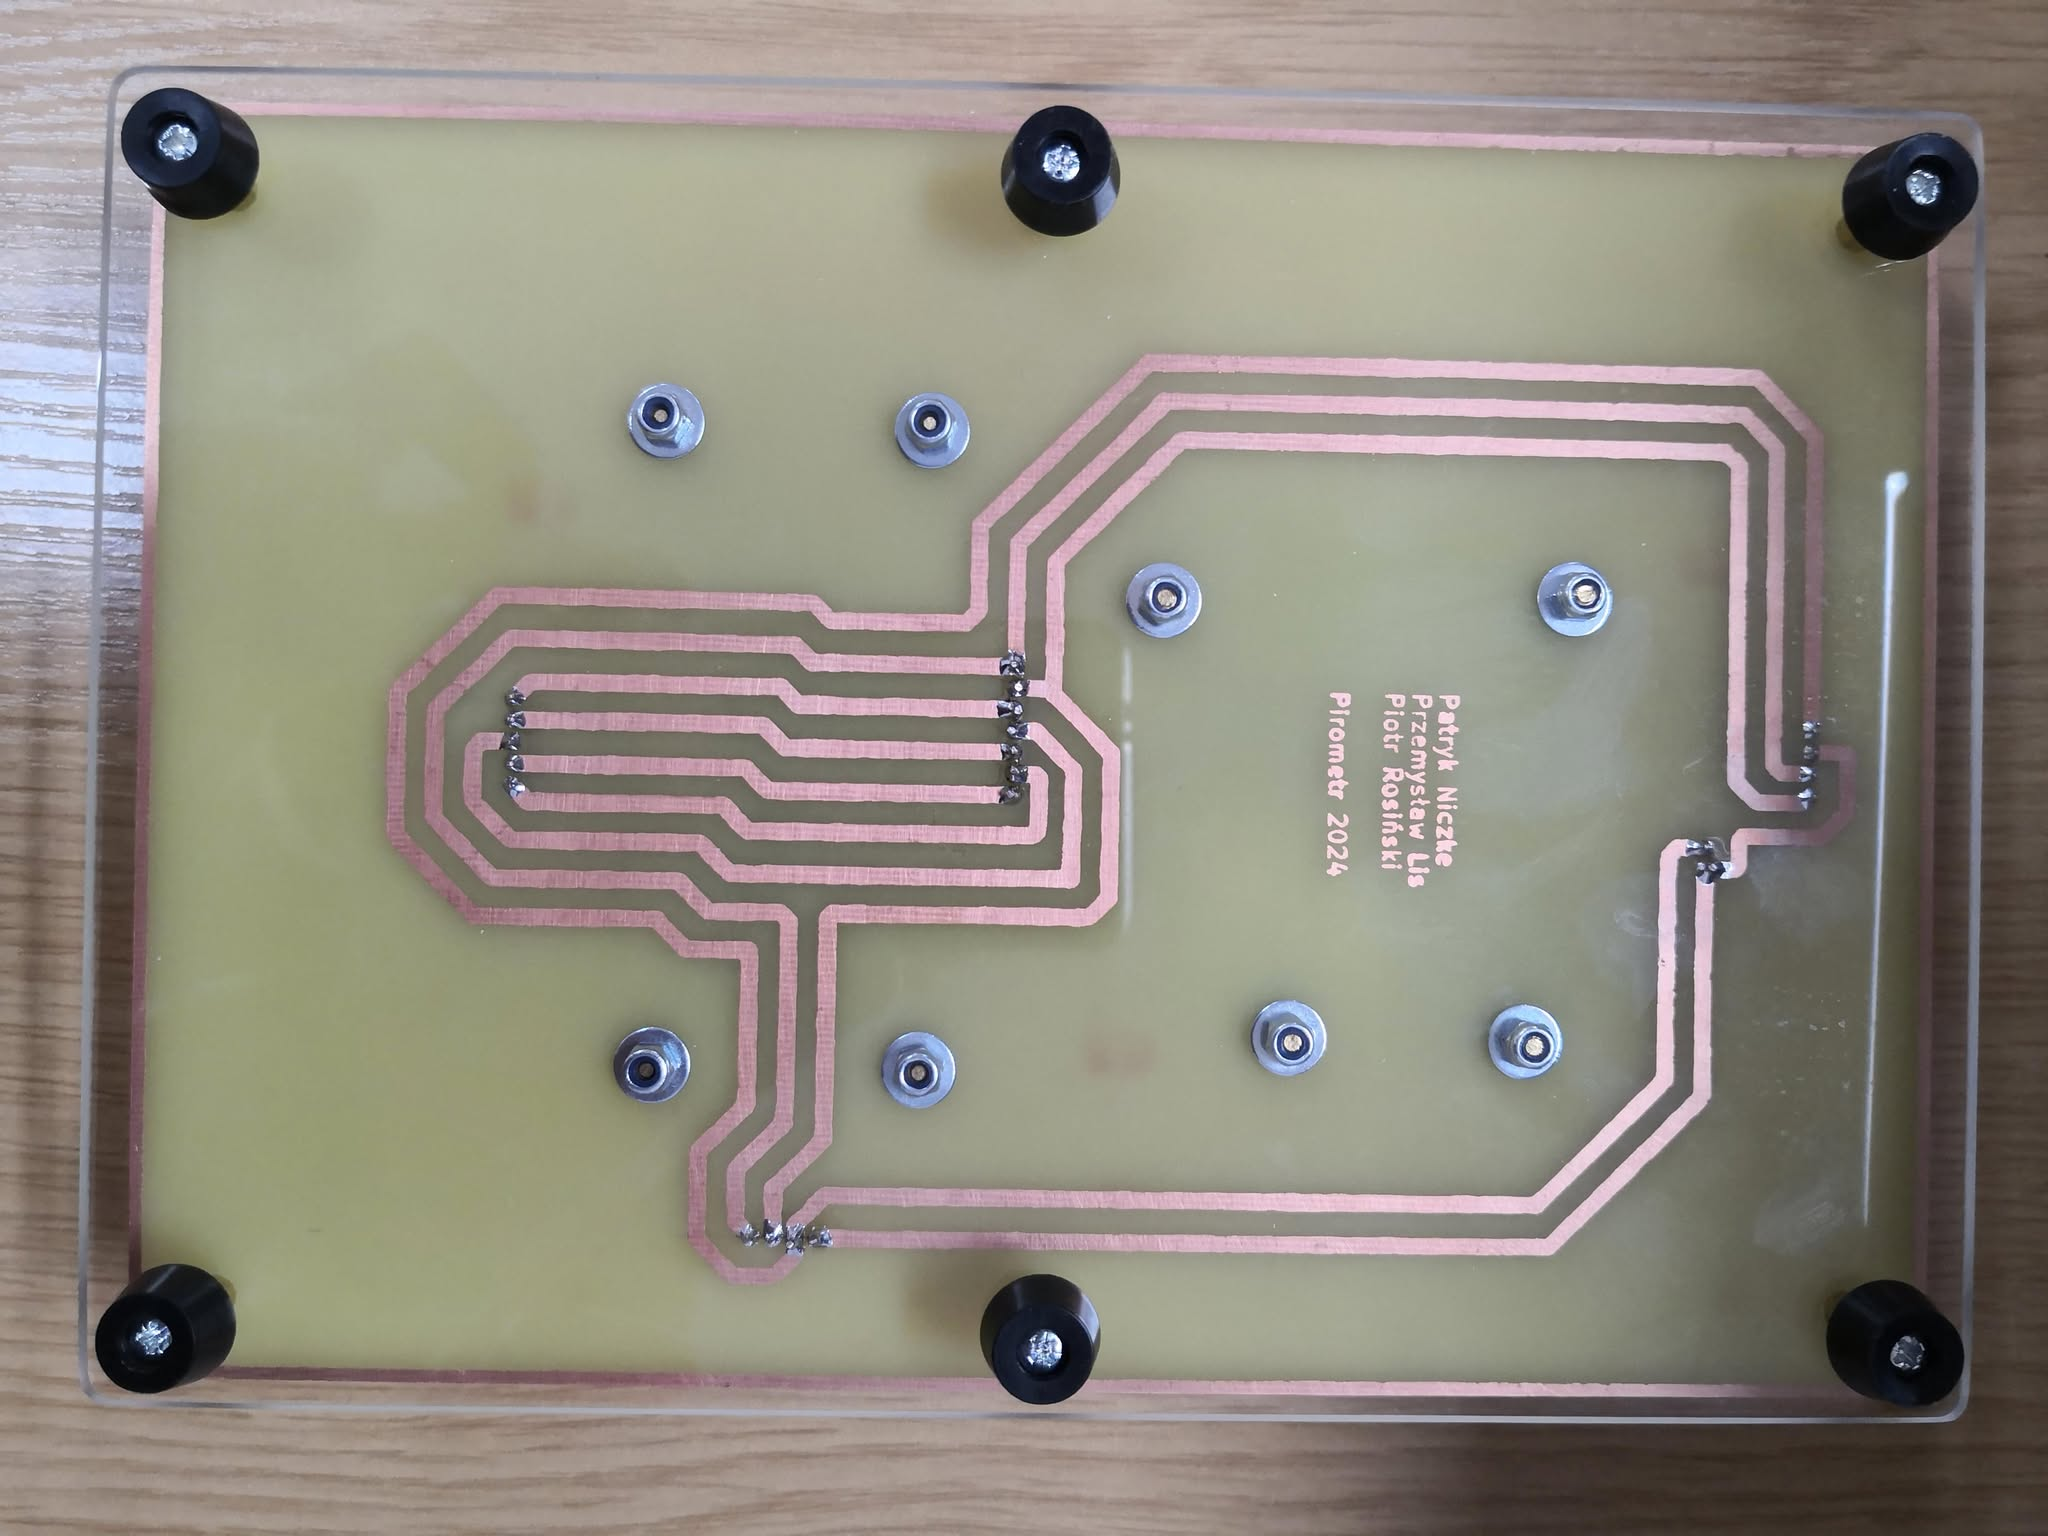
\includegraphics[width=0.9\textwidth]{images/tyl.jpg}
    \caption{Panel tylny urządzenia}
    \label{fig:panel_gorny}
\end{figure}

\begin{figure}[h!]
    \centering
    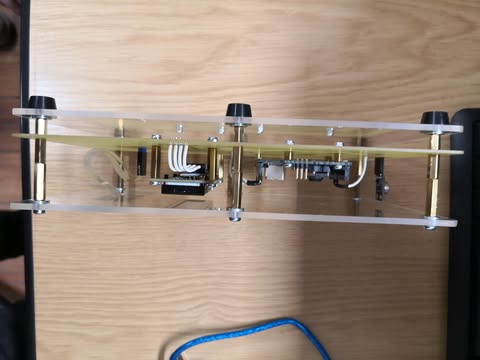
\includegraphics[width=0.85\textwidth]{images/bok2.jpg}
    \caption{Widok z boku}
    \label{fig:panel_gorny}
\end{figure}

\begin{figure}[h!]
    \centering
    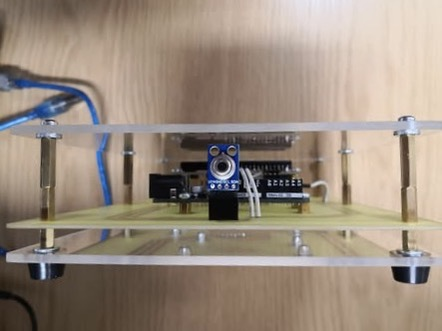
\includegraphics[width=0.8\textwidth]{images/bok3.jpg}
    \caption{Widok z boku}
    \label{fig:panel_gorny}
\end{figure}

\begin{figure}[h!]
    \centering
    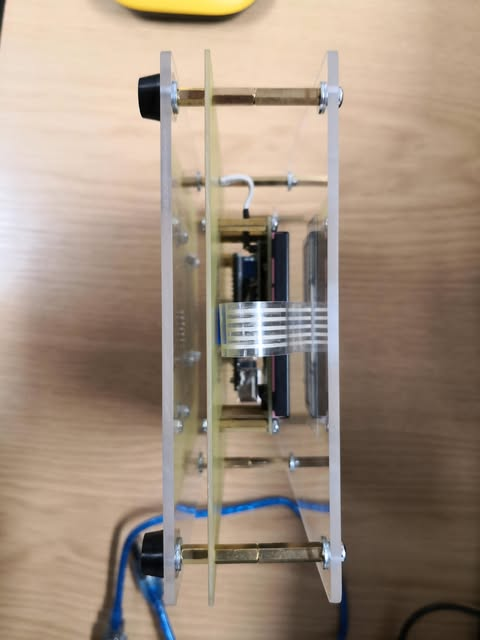
\includegraphics[width=0.6\textwidth]{images/bok4.jpg}
    \caption{Widok z boku}
    \label{fig:panel_gorny}
\end{figure}

%\section{Ostrzeżenia dotyczące pomiarów  wysokich temperatur/kontaktu z gorącymi obiektami}
%\section{Podłączenie pirometru do źródła zasilania}
%\section{Opcjonalna zmiana parametrów (emisyjność, odległość dokonywania pomiaru)}
%\section{Informacje o przechowywaniu}
%\section{Typowe problemy (np. brak odczytu, błędne wyniki) i ich możliwe rozwiązania}